\documentclass[11pt]{article}
\usepackage{fancyhdr}
\usepackage[usenames, dvipsnames]{xcolor}
\usepackage{graphicx,hyperref}
\hypersetup{
	colorlinks,
	citecolor=black,
	filecolor=black,
	linkcolor=black,
	urlcolor=black
}
\newcommand{\HRule}{\rule{\linewidth}{0.5mm}}
\pagestyle{fancy}
\lfoot{\small \color{gray}Tom Peerdeman - 10266186}
\cfoot{\thepage}
\rfoot{\small \color{gray}Ren\'e Aparicio Sa\'ez - 10214054}
\lhead{\small \color{gray}Opgave 3: Geheugenbeheer}
\begin{document}
	\begin{titlepage}
	\begin{center}
		\textsc{\Large Besturingssystemen}\\[0.5cm]
		\HRule \\[0,4cm]
		\textsc{\huge \bfseries Geheugenbeheer}
		\HRule \\[8cm]
		\begin{minipage}{0.4\textwidth}
			\begin{flushleft}\large
				\emph{Auteurs: Tom Peerdeman \& Ren\'e Aparicio Saez}\\
			\end{flushleft}
		\end{minipage}
		\begin{minipage}{0.4\textwidth}
			\begin{flushright}\large
			\emph{Datum: 03f-06-2012\\\'}\\
			\end{flushright}
		\end{minipage}
	\end{center}
	\end{titlepage}

	\tableofcontents
	\newpage

	\section{Inleiding}\label{sec:inleiding}
	Geheugenbeheer en de allocatie van geheugen is erg belangrijk binnen een computer. Het moet op een functionele manier gebeuren en het geheugen moet optimaal benut worden. Geheugen-allocatie kan op vele verschillende manieren worden afgehandeld. Specifiek wordt er gekeken naar de wost-fit methode en de first-fit methode.\\[4cm]
	\begin{figure}[h]
		\begin{center}
		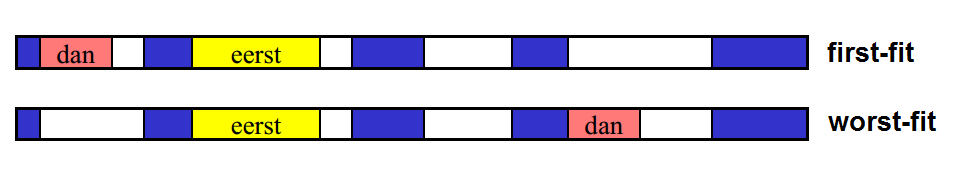
\includegraphics[width=1\textwidth]{geheugenbeheer.png}
		\caption{Schematische weergave van First-fit en Worst-fit}
		\end{center}
	\end{figure}

	\newpage


	\section{First-fit}\label{sec:first-fit}
	\subsection{Inleiding first-fit}\label{sec:inleidingff}
	De allocatie van geheugen bij first-fit, werkt zoals de naam al doet denken. De eerst mogelijke plaatst waar het stuk geheugen gealloceerd zou kunnen worden wordt ook gealloceerd. De allocatie is over het algemeen erg snel en hierdoor is first-fit een goed werkend geheugenbeheer algoritme.


	\section{Worst-fit}\label{sec:worst-fit}
	\subsection{Inleiding worst-fit}\label{sec:inleidingwf}
	De allocatie van geheugen bij worst-fit zoekt het grootste vrije blok geheugen op. Als dit blok is gevonden wordt daar het geheugen gealloceerd. Dit algoritme is bedacht om wat grotere stukken geheugen vrij te laten bij het alloceren. Als een stuk vrij geheugen groot is, dan is er een grotere kans dat het nog gebruikt kan gaan worden. Hele kleine stukken geheugen kunnen namelijk over het algemeen niet worden toegewezen. Het worst-fit algoritme werkt iets langzamer omdat het moet bijhouden hoe groot ieder vrij stuk is en moet bepalen waar het grootste vrije stuk zich bevind.


	\section{Makefile / setup}\label{sec:makefile}
	De makefile maakt twee programma's: worst-fit en first-fit. Om de programma's te maken dient het commando 'make' uitgevoerd te worden. De programma's worden dan gecompileerd en gelinkt. Om beide programma's snel achter elkaar te runnen moet eerst de directory 'out' worden gemaakt. Dit kan door middel van het commando 'make setup' uit te voeren. Vervolgens worden doormiddel van het commando 'make run' beide programma's uitgevoerd. De input die aan de programma's meegegeven wordt staat in de file 'input.txt' in de directory 'input'. De output die het programma geeft wordt weggeschreven naar 'worst-fit.txt' of 'first-fit.txt' in de directory out. Om de output snel te verwijderen kan het commando 'make cleanout' worden uitgevoerd. De uitvoer bestanden worden dan verwijderd. Om alle gecompileerd en gelinkt files te verwijderen kan het commando 'make clean' gebruikt worden. Om zowel de outputfiles als de gecompileerde en gelinkte files te verwijderen kan het commando 'make cleanall' gebruikt worden.

	\section{Resultaten}\label{sec:resultaten}


\end{document}
